\documentclass[12pt]{article}

% a template that a friend gave, it's worked well enough for me
% i have added some packages and stuff that have proved useful

\usepackage{fancyhdr}
\usepackage{tipa}
\usepackage{fontspec}
\usepackage{amsfonts}
\usepackage{enumitem}
\usepackage[margin=1in]{geometry}
\usepackage{graphicx}
\usepackage{float}
\usepackage{amsmath}
\usepackage{braket}
\usepackage{amssymb}
\usepackage{booktabs}
\usepackage{hyperref}
\usepackage{mathtools}
\usepackage{xcolor}
\usepackage{float}
\usepackage{algpseudocodex}
\usepackage{titlesec}
\usepackage{bbm}

\pagestyle{fancy}
\fancyhf{} % sets both header and footer to nothing
\lhead{Kevin Sheng}
\setmainfont{Comic Neue}
\renewcommand{\headrulewidth}{1pt}
\setlength{\headheight}{0.75in}
\setlength{\oddsidemargin}{0in}
\setlength{\evensidemargin}{0in}
\setlength{\voffset}{-.5in}
\setlength{\headsep}{10pt}
\setlength{\textwidth}{6.5in}
\setlength{\headwidth}{6.5in}
\setlength{\textheight}{8in}
\renewcommand{\headrulewidth}{0.5pt}
\renewcommand{\footrulewidth}{0.3pt}
\setlength{\textwidth}{6.5in}
\usepackage{setspace}
\usepackage{multicol}
\usepackage{float}
\setlength{\columnsep}{1cm}
\setlength\parindent{24pt}
\usepackage [english]{babel}
\usepackage [autostyle, english = american]{csquotes}
\MakeOuterQuote{"}

\setlength{\parskip}{6pt}
\setlength{\parindent}{0pt}

\titlespacing\section{0pt}{12pt plus 4pt minus 2pt}{0pt plus 2pt minus 2pt}
\titlespacing\subsection{0pt}{12pt plus 4pt minus 2pt}{0pt plus 2pt minus 2pt}
\titlespacing\subsubsection{0pt}{12pt plus 4pt minus 2pt}{0pt plus 2pt minus 2pt}

\hypersetup{colorlinks=true, urlcolor=blue}

\newcommand{\correction}[1]{\textcolor{red}{#1}}


\begin{document}
\begin{enumerate}
    \item By Euler's formula,
          \begin{align*}
              e^{(1+i)t}\begin{bmatrix}-1+i \\ 2\end{bmatrix} & = e^t e^{ti}\begin{bmatrix}-1+i \\ 2\end{bmatrix}              \\
                                                              & = e^t(\cos t + i \sin t) \begin{bmatrix}-1+i \\ 2\end{bmatrix} \\
                                                              & = e^t \begin{bmatrix}
                                                                          -\sin t - \cos t + i(\cos t - \sin t) \\
                                                                          2\cos t + 2i \sin t
                                                                      \end{bmatrix}
          \end{align*}
          By inspection, we can see that the real and imaginary part of the solution are
          \[e^t \begin{bmatrix}
                  -\sin t - \cos t \\ 2 \cos t
              \end{bmatrix} \text{ and } e^t \begin{bmatrix}
                  \cos t - \sin t \\ 2\sin t
              \end{bmatrix}\]
          repsectively.
    \item The characteristic polynomial of $A$ is
          \[\det \begin{bmatrix}
                  -1-\lambda & 3          \\
                  -3         & -1-\lambda
              \end{bmatrix}=(-1-\lambda)^2+9=\lambda^2+2\lambda+10\]
          Plugging this into the quadratic formula, we get that the eigenvalues of $A$ are $-1 \pm 3i$.
          Choosing one of them and evaluating to find $\vec{v}$, we see that
          \[\begin{bmatrix}a \\ b\end{bmatrix} \cdot (-1+3i)=\begin{bmatrix}-1 & 3 \\ -3 & -1\end{bmatrix}\begin{bmatrix}a \\ b\end{bmatrix}\]
          and a particular solution to this (as there are infinitely many) is $a=-i$ and $b=1$.
          Now, we plug these two values into $e^{-t\lambda}\vec{v}$ to get
          \begin{align*}
              e^{t(-1+3i)} \begin{bmatrix}i \\ 1\end{bmatrix} & = e^{-t} e^{3ti} \begin{bmatrix}-i \\ 1\end{bmatrix}                \\
                                                              & = e^t (\cos (3t) + i \sin (3t)) \begin{bmatrix}-i \\ 1\end{bmatrix} \\
                                                              & = e^t \begin{bmatrix}
                                                                          \sin (3t)-i \cos (3t) \\
                                                                          \cos (3t)+i \sin (3t)
                                                                      \end{bmatrix}
          \end{align*}
          and then our fundamental set of solutions
          \[y_1=\begin{bmatrix}
                  e^t \sin(3t) \\
                  e^t \cos(3t)
              \end{bmatrix} \qquad y_2=\begin{bmatrix}
                  -e^t \cos (3t) \\
                  e^t \sin (3t)
              \end{bmatrix}\]
          Solving for initial conditions, we finally get our solution
          \[y=2\begin{bmatrix}
                  e^t \sin(3t) \\
                  e^t \cos(3t)
              \end{bmatrix}-3\begin{bmatrix}
                  -e^t \cos (3t) \\
                  e^t \sin (3t)
              \end{bmatrix}\]

          \pagebreak

    \item The only eigenvalue is $\lambda=-2$, and its corresponding eigenvector is $\begin{bmatrix}
        1 \\ 1
    \end{bmatrix}$.
    It remains to find a vector $\vec{v}$ s.t. $(A-\lambda I)\vec{v}=\begin{bmatrix}
        1 \\ 1
    \end{bmatrix}$.
    Setting up this to be solved, we find that
    \[\begin{bmatrix}
        -3-(-2) & 1 \\
        -1 & -1-(-2)
    \end{bmatrix}\begin{bmatrix}
        a \\ b
    \end{bmatrix}=\begin{bmatrix}
        1 \\ 1
    \end{bmatrix}\]
    and solving, we get a particular solution $a=0$ and $b=1$.

    Thus, our fundamental set of solutions are
    \begin{gather*}
        y_1 = e^{-2t}\begin{bmatrix}1 \\ 1\end{bmatrix} \\
        y_2 = e^{-2t}\left(\begin{bmatrix}0 \\ 1\end{bmatrix}+t\begin{bmatrix}1 \\ 1\end{bmatrix}\right)
    \end{gather*}
    and combining these two into a linear combination gives us our general solution

    \[y=C_1e^{-2t}\begin{bmatrix}1 \\ 1\end{bmatrix}+C_2e^{-2t}\left(\begin{bmatrix}0 \\ 1\end{bmatrix}+t\begin{bmatrix}1 \\ 1\end{bmatrix}\right)\]

    \item The first solution moves toward the origin, while the second one moves away.
    \begin{center}
        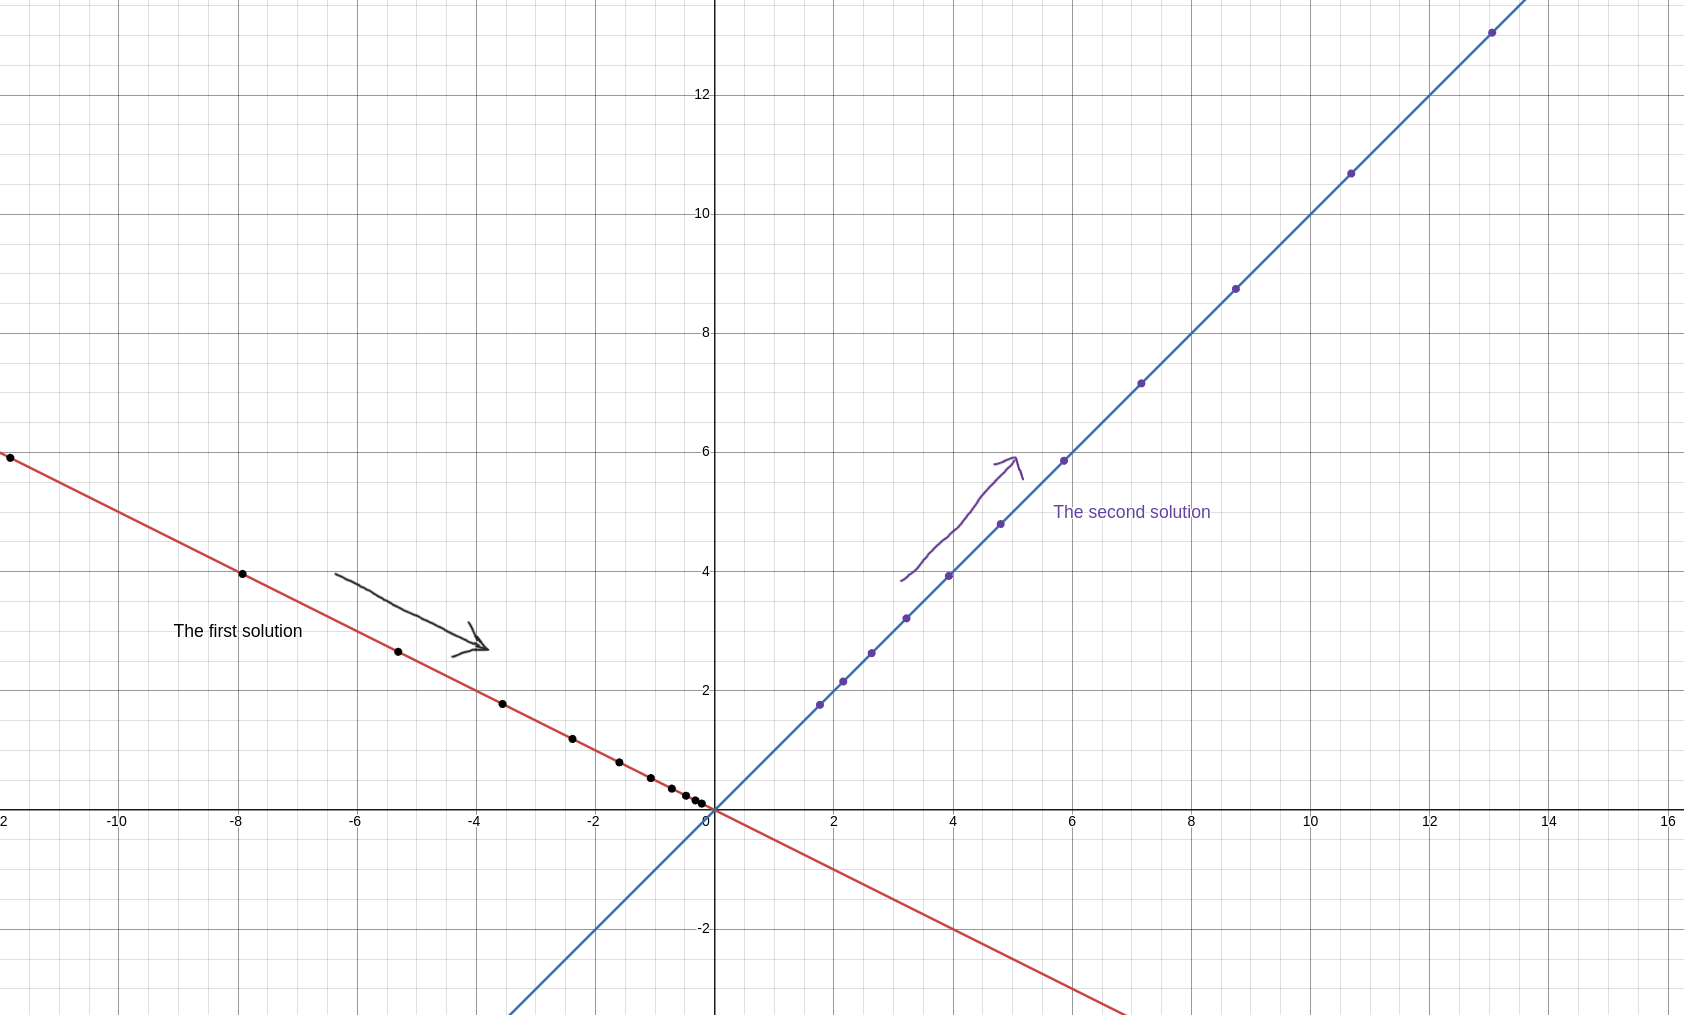
\includegraphics[width=15.4cm]{img/phase}
    \end{center}

    \item We first find the generalized eigenvector for $\lambda_1=3$:
          \begin{gather*}
              \begin{bmatrix}
                  3-3 & 1 & 0 \\
                  0 & 3-3 & 2 \\
                  0 & 0 & 5-3   
              \end{bmatrix}\begin{bmatrix}a \\ b \\ c\end{bmatrix}=
              \begin{bmatrix}1 \\ 0 \\ 0\end{bmatrix}
          \end{gather*}
          Solving this, we get that $a=c=0$ and $b=1$, so the generalized eigenvector is $\boxed{\begin{bmatrix}0 \\ 1 \\ 0\end{bmatrix}}$.

          Plugging this into the formula for the general solution, we have
          \[\vec{y}=C_1e^{3t}\begin{bmatrix}
            1 \\ 0 \\ 0
          \end{bmatrix}+C_2e^{5t}\begin{bmatrix}
            1 \\ 2 \\ 2
          \end{bmatrix}+C_3\left(e^{3t}\begin{bmatrix}
            0 \\ 1 \\ 0
          \end{bmatrix}+te^{3t}\begin{bmatrix}
            1 \\ 0 \\ 0
          \end{bmatrix}\right)\]

    \item The characteristic polynomial of $A$ is
          \begin{align*}
              \det \begin{bmatrix}
                       a-\lambda & b         \\
                       c         & d-\lambda
                   \end{bmatrix} & = (a-\lambda)(d-\lambda)-bc          \\
                                       & = \lambda^2-\lambda(a+d)+ad-bc
          \end{align*}
          By the quadratic formula, the roots of this polynomial are
          \[\lambda=\frac{(a+d) \pm \sqrt{(a+d)^2-4(ad-bc)}}{2}\]
          There are three cases to consider.

          $\mathbf{4(ad-bc) < (a+d)^2}$ \\
          In this case, the discriminant is positive and we have two distinct real
          roots of the quadratic.
          $(a+d)-\sqrt{\text{''}}$ is negative because $a+d<0$ and $\sqrt{x}>0$,
          while $(a+d)+\sqrt{\text{''}}$ is also negative because
          \begin{align*}
              0       & >(a+d)+\sqrt{\text{''}}   \\
              -(a+d)  & > \sqrt{(a+d)^2-4(ad-bc)} \\
              (a+d)^2 & > (a+d)^2-4(ad-bc)        \\
              0       & > -4(ad-bc)               \\
              0       & < ad-bc
          \end{align*}
          which we know to be true by the premise.
          Notice that we could square both sides of the inequality since both sides
          were positive there.

          Thus, any solution to this diffeq must have $e^{cx}$ as a coefficient,
          where $c<0$ as both eigenvalues must be negative.
          $\lim_{x \to \infty} e^{cx}=0$, so this solution must tend to $\vec{0}$ as well.

          $\mathbf{4(ad-bc) > (a+d)^2}$: \\
          Here, $\lambda$ takes the form of a complex number $x \pm yi$, where $x=\frac{a+d}{2} < 0$.
          By Euler's formula, we know
          \[e^{t(x \pm yi)}=e^{xt} \cdot e^{\pm tyi}=e^{xt}(\cos(yt)+i\sin(yt))\]
          All solutions then must have a coefficient $e^{xt}$ in each of their vector elements,
          which tends to $0$ since $x < 0$.
          Thus, the solution must tend to $\vec{0}$ as $t$ gets large.

          $\mathbf{4(ad-bc) = (a+d)^2}$: \\
          The final solution for this case takes the form
          \[y(t)=e^{\lambda t}\left(C_1\vec{v_1}+C_2\left(t\vec{v_1}+\vec{v_2}\right)\right)\]
          where $\lambda=\frac{a+d}{2}<0$.
          By inspection, it's clear that as $t$ gets larger, $e^{\lambda t} \to 0$
          and the whole solution goes to $\vec{0}$. $\square$
\end{enumerate}
\end{document}
